% !TEX root =  ./main.tex

\subsection{Comorbidity Treatment Analysis}\label{sec:cmsb2024}

%The paper~\cite{DBLP:conf/cmsb/BowlesBBFGM24} introduced the notion of RS with guarded contexts, recalled in \Cref{sec:RS}.
%to model scenarios where the entities to be provided by the context are dependent upon the current state, which is a common situation arising, e.g., in drug administration and \emph{in silico} experiments. 
This case was studied in~\cite{DBLP:conf/cmsb/BowlesBBFGM24}, where guarded contexts were introduced to handle key features of medical treatments. It concerns the risk mitigation of medication harm in the treatment of patients with comorbidities; i.e., patients with two or more long-term chronic conditions (such as diabetes, hypertension, cardiovascular diseases, chronic kidney disease, cancer, chronic obstructive pulmonary disease, among many others), who are therefore subject to follow several treatment plans simultaneously, called \emph{clinical guidelines}~\cite{feder1999using,woolf1999potential}. Since clinical guidelines address a single disease, comorbidities easily lead to  \emph{polypharmacy}, where 5 or more medications must be administered, increasing the risk of adverse drug reactions, or of making certain drugs less effective when combined~\cite{Gut12}. 

\subparagraph*{Analysis goals.}
The goal of the analysis is to explore the combination of clinical guidelines in the presence of comorbidities and for different patient profiles to detect if major risks can arise from the treatments and which profiles are exposed at severe risks.
Using formal methods for risk mitigation intends to help doctors choose between alternative treatment options as well as to point out missing conditions that could be helpful to revise and update clinical guidelines. 

\subparagraph*{Features of interest.}
In this case study, reachability and causal analysis are key issues.
Specifically, reachability is used to address questions such as \emph{can the combination of clinical guidelines expose the patient at serious risks because of drugs interference?}
Then, in the affirmative case, causal analysis can help to detect which medical decisions would be directly responsible for causing serious harm as well as to point out  which alternative treatment would be available, if any.
We selected this case study because the use of guarded contexts introduces new challenges for the causal analysis of RSs: while existing approaches typically focus on identifying combinations of drugs administered within the context that may have caused harm, they often fail to highlight the medical decisions that led to their administration.

\subparagraph*{Experimental set up.}
The RS encoding proposed in~\cite{DBLP:conf/cmsb/BowlesBBFGM24} relies on a formal representation of patient profiles, medical guidelines and adverse drug reactions.

For each drug $d$ that appears in the therapies, we consider three corresponding entities $\mathsf{get}\_d$, $\mathsf{stop}\_d$  and $d$: the first represents the prescription of $d$ by the doctor, the second the removal of $d$ from the current treatment and the third the intake of the drug by the patient. For handling multiple drugs of the same class $c$, we exploit analogous entities $\mathsf{stop}\_c$  and $c$.

For medical guidelines, it takes in input the event structure modelling of therapies introduced in~\cite{BC17c}. Roughly, to each event $e$ there is an identifier $\mathsf{E}_e$ defined as a sum of processes, one for each outgoing arc of $e$. If some guard is attached to the arc, then the corresponding alternative is also guarded. The prescription of a drug $d$ is modelled by the provision of the entity $\mathsf{get}\_d$. Similarly, if the therapy requires stopping the drug $d$, the entity $\mathsf{stop}\_d$ is produced.

The patient profile is determined by the conditions that trigger the treatment (e.g., headache, hypertension) and by the conditions that appear in the arc labels of the event structure (e.g., pregnant, asthma). We call them \emph{features}. Correspondingly, there is one context $\mathsf{K}_f = \{f\}.\mathsf{Emp}$ for each feature $f$, and a patient profile is just a combination of features $\prod_f \mathsf{K}_f$. 
Once the profile is determined by the context, it is preserved during the rest of the computation by reactions of the form $(\{f\},\varnothing,\{f\})$, one for each feature.
Accounting for all possible combination of features in a single model can be done by considering the context $\prod_f (\mathsf{K}_f + \mathsf{Emp})$. 

For each drug $d$ of class $c$, there will be the following reactions: $(\{\mathsf{get}\_d\},\{\mathsf{stop}\_d,\mathsf{stop}\_c\},\{d,c\})$ modelling the intake of the drug $d$ as for doctor prescription, and $(\{d\},\{\mathsf{stop}\_d,\mathsf{stop}\_c\},\{d,c\})$ modelling the prosecution of the therapy.
Adverse drug reactions are provided in the form of so-called ADR tables.
Each row corresponds to a set of medications $M$, a textual description of their side effects and risks when used in combination, and a severity level $m$ (e.g., \minor, \moderate, \major).
Each row translates to a reaction $(M,\varnothing,\{m\})$. 

\subparagraph*{Previous approach.}
The approach outlined in~\cite{DBLP:conf/cmsb/BowlesBBFGM24} has been used to synthesize the patient profiles that are more at risk, as a support for dynamic guideline revision: by refining guarded contexts to prevent severe effects for specific patients, we can readily check the efficacy of the changes.

\subparagraph*{\GROOVE experimentation.}

The benefit of using \GROOVE in this case study is that, besides identifying situations where a risk is found, for any risk so identified the corresponding occurrence graph of a risk can be generated, using the process outlined in \Cref{sec:RS2GTS}. This provides a means for medical experts to more easily analyze root causes: for any risk that has been identified, what is the causal structure of the steps and entities leading up to it?

\GROOVE can be used for full state space generation, for instance to count the number of ways a minor, moderate or major risk can arise. Some statistics can be found in \Cref{tab:cmsb-experiments}.

\begin{figure}\centering
\subcaptionbox{Full exploration\label{fig:cmsb-full}}{
\begin{tabular}{lcrr}
\bf Measurement & \bf Search & \bf Count & \bf Time \\
                & \bf method & \bf       & \bf  (s) \\
\hline\hline
Total states   & BFS & 309 798 & 3 368 \\
Total states   & DFS & 309 798 & 2 464 \\
\hline
Major risks    & DFS &  91 113 & 2 447 \\
Moderate risks & DFS &  97 805 & 1 534 \\
Maj\&Mod risks & DFS &  61 976 & 2 727 \\
Minor risks    & DFS &      24 & 2 218
\end{tabular}}

\subcaptionbox{Bounded BFS exploration of major risks (tabular)\label{fig:cmsb-steps}}{
\begin{tabular}{rrrrr}
\bf Explore & \bf Total & \bf New   & \bf Total    & \bf New    \\ % & \bf Time
\bf depth   & \bf risks & \bf risks & \bf states & \bf states \\ % & \bf  (s)
\hline\hline
 1 &      0 &       0 &     769 &     769 \\ % &     3
 2 &      0 &       0 &   1 345 &     576 \\ % &     3
 3 &      0 &       0 &   1 873 &     528 \\ % &     3
 4 &    716 &     716 &   8 133 &   6 260 \\ % &    10
 5 &  9 317 &   8 601 &  42 293 &  34 160 \\ % &    70
 6 & 35 899 &  26 582 & 126 012 &  83 719 \\ % &   425
 7 & 73 591 &  37 693 & 227 866 & 101 854 \\ % & 2 277
 8 & 81 691 &   8 100 & 248 420 &  20 554 \\ % & 1 765
 9 & 88 631 &   6 940 & 276 924 &  28 504 \\ % & 1 875
10 & 89 733 &   1 102 & 281 854 &   4 930 \\ % & 2 368
11 & 90 573 &     840 & 286 054 &   4 200 \\ % & 2 443
12 & 91 133 &     560 & 288 854 &   2 800
   % & 2 784
\end{tabular}}
\subcaptionbox{Bounded BFS exploration of major risks (chart)\label{fig:cmsb-trends}}{
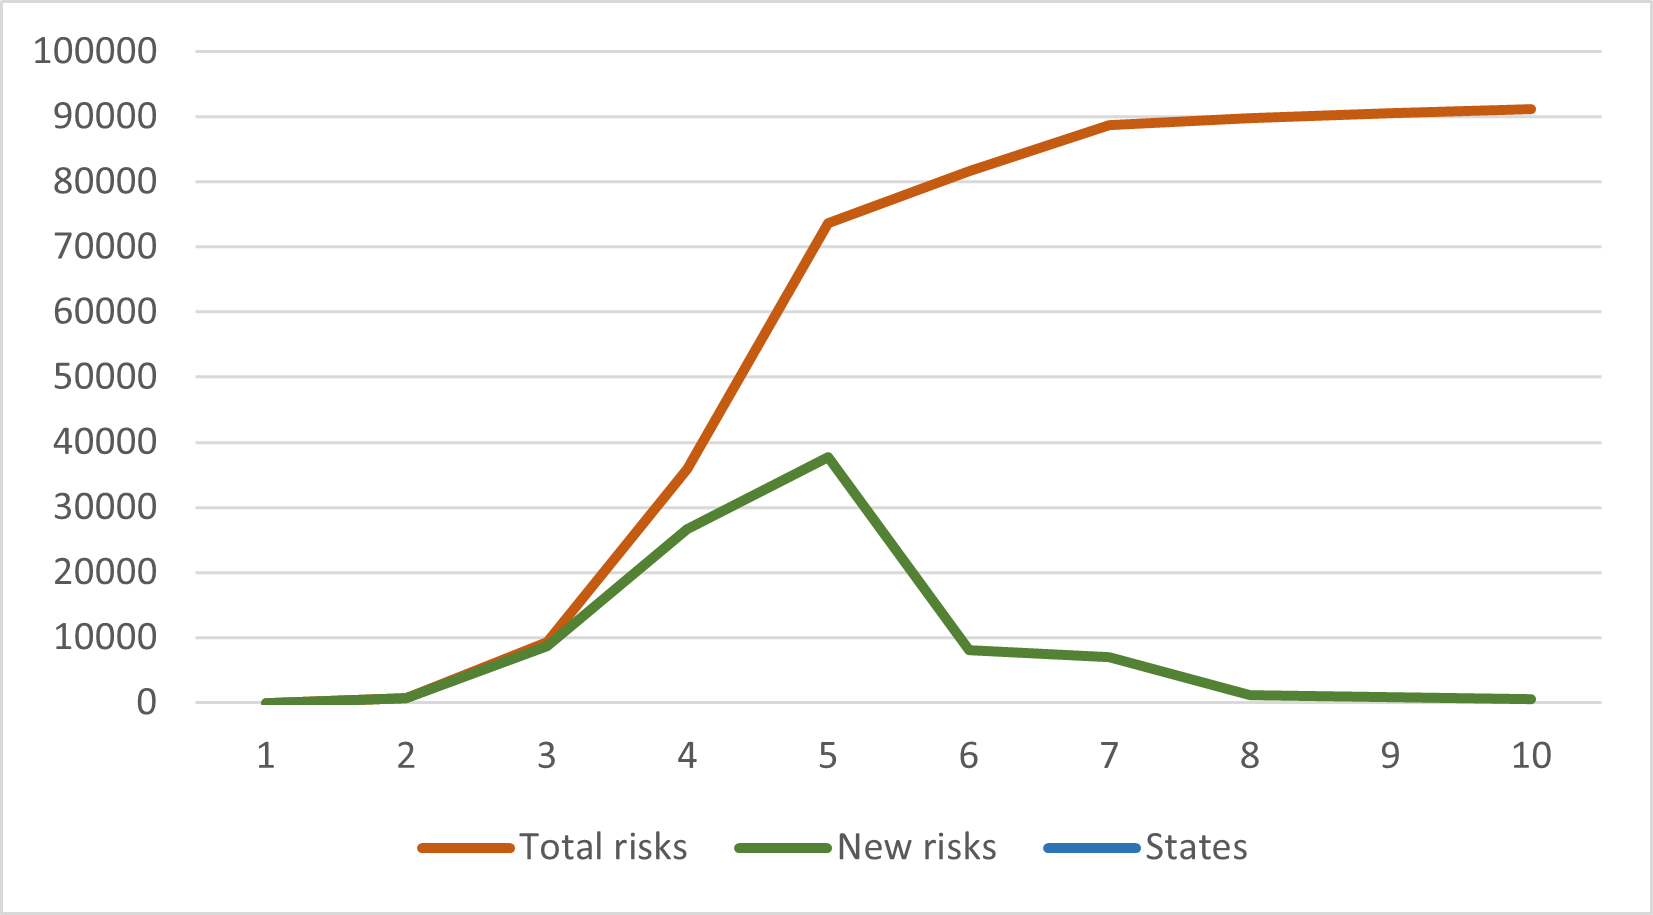
\includegraphics[scale=.6]{figs/cmsb-trends}}
\caption{States, risks and execution time}
\label{tab:cmsb-experiments}
\end{figure}

The first two lines show that depth-first exploration strategy (DFS) is generally more convenient than breadth-first (BFS), so we rely on the former for the subsequent entries. At first sight, the number of major (and moderate) risks reported in \Cref{tab:cmsb-experiments} seems impossibly large, and evidently implies that there are patient profiles that give rise to many risks. However, this should be interpreted with care: the count refers to the total number of configurations containing a \Forbidden (i.e., \major or \minor) entity, and there may very well be entities whose presence or absence does not causally contribute to that \Forbidden entity --- in other words, which would not appear in its occurrence graph. Configurations counted as separate risks may well reduce to the same causation. To analyse this further, one would have to construct (and prune) the occurrence graphs for all risk configurations, and compare them on that basis. Though this is beyond the scope of this paper, such an analysis is in principle straightforward to carry out in \GROOVE --- it is a matter of combining the three steps in \Cref{fig:chain} into a single rule system.

The line of \Cref{fig:cmsb-full} headed ``Maj\&Mod risks'' reports the number of configurations at which \emph{both} a \major and a \moderate entity appear during the same step; hence, these are counted as both major and moderate risks (partially explaining their high numbers).
 
\medskip\noindent By exploring only up to a certain depth, we can get some idea of the number of steps after which a risk typically appears, which in turn indicates the complexity of the context in which it appears. \Cref{fig:cmsb-steps} shows how many major risks occur after a fixed number of reaction steps, and also how much of the total state space is involved. Note that, in this case, the total state count (reached after 12 steps) stays below that of \Cref{fig:cmsb-full}; this is because in the experiments of \Cref{fig:cmsb-steps} we stop exploration at states where a risk has been found. \Cref{fig:cmsb-trends} shows the same data in a graphical form.

\medskip\noindent Alternatively, we can stop exploring after having found a predetermined number of risks. By setting the exploration strategy to breadth-first search, it is guaranteed that the risks found are those reached after the shortest number of steps, meaning they are the easiest to analyze visually. For instance, \Cref{fig:cmsb-pruned} shows the occurrence graph of the first major risk found in this way.

\begin{figure}
\centering
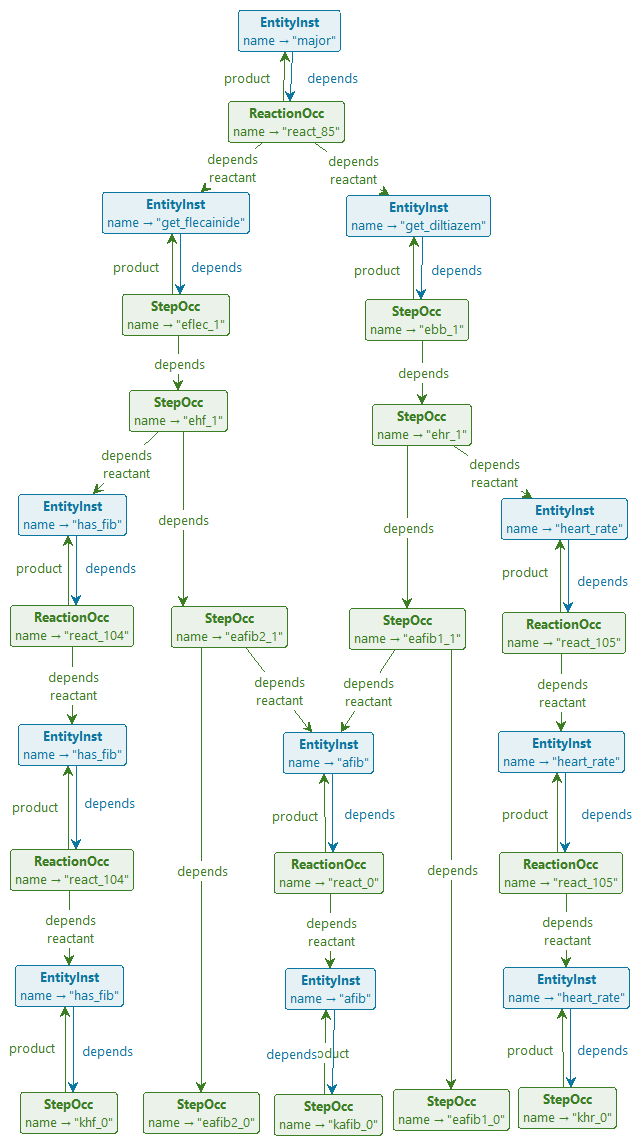
\includegraphics[scale=.3]{./figs/cmsb-pruned}
\caption{Occurrence graph of a major risk}
\label{fig:cmsb-pruned}
\end{figure}

The patient configuration in question is a combination of \texttt{has\_fib}, \texttt{afib} and \texttt{heart\_rate}; the combination of the first two leads to the prescription of \texttt{fleacinide} and the second to the prescription of \texttt{diltiazem}, the combination of which should, however, be avoided. By counting the longest chain of \StepOcc-nodes, it is confirmed that it indeed takes 4 steps to establish this risk.

\medskip\noindent We can also use \GROOVE to replicate the findings of \cite[Fig.~6]{DBLP:conf/cmsb/BowlesBBFGM24} in terms of the relation between patient profiles and risks, using model checking. Recall that the reaction system starts by having the context produce initial entities, and in this particular case study, the first move of the context is to select a patient profile; hence the initial state has $2^9=512$ outgoing transitions, whose target state corresponds to the chosen profile. Moreover, the rule \forbidden tests for the presence of a \Forbidden entity in a state. Therefore, a formula of the shape
$\AX(\bigwedge_i f_i \rightarrow \EF \forbidden)$, where each of the $f_i$ specifies the presence or absence of a patient feature, specifies whether all patient profiles with that combination of features contain a potential risk.

Concretely, in the case study at hand, \cite[Fig.~6]{DBLP:conf/cmsb/BowlesBBFGM24} contains necessary and sufficient criteria for patient profiles to contain major, moderate and minor risks. The part of the table pertaining to major risks is reproduced in \Cref{fig:table-from-cmsb2024}. This should be read as: \emph{precisely} in the combination of features where the green ones are present and the red ones absent, a major risk may occur.
%
\begin{figure*}
\centering
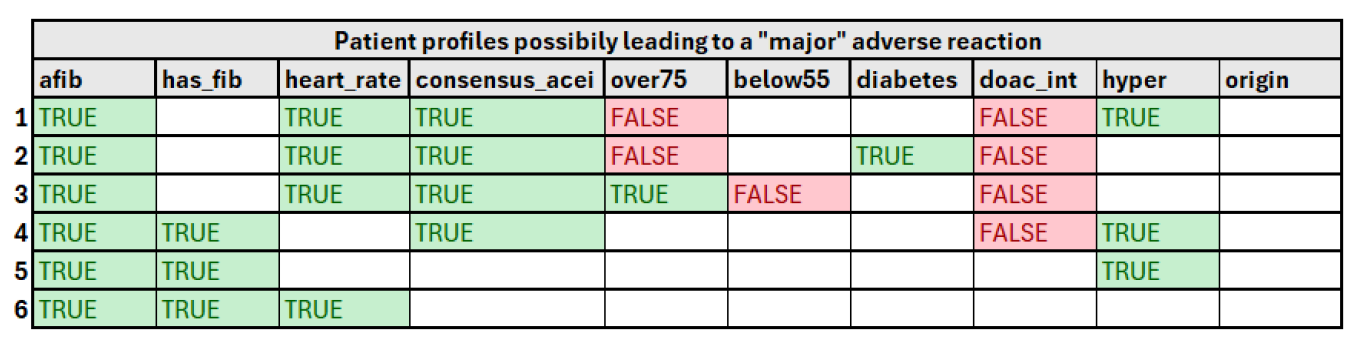
\includegraphics[scale=.4]{./figs/table-from-cmsb2024}\begin{lstlisting}[basicstyle=\ttfamily\small,xleftmargin=0cm]
AX( (afib           & heart_rate & consensus_acei & !over75                       & !doac_int & hyper |
     afib           & heart_rate & consensus_acei & !over75            & diabetes & !doac_int         |
     afib           & heart_rate & consensus_acei &  over75 & !below55            & !doac_int         |
     afib & has_fib              & consensus_acei                                 & !doac_int & hyper |
     afib & has_fib                                                                           & hyper |
     afib & has_fib & heart_rate                                                                      )
   <-> EF forbidden)
\end{lstlisting}
\caption{CTL encoding of the major risk profiles found in \cite[Fig.~6]{DBLP:conf/cmsb/BowlesBBFGM24}}
\label{fig:table-from-cmsb2024}
\end{figure*}

In order to replicate these results, we can use CTL model checking. For instance, the relevant CTL property for the major risks is also shown in \Cref{fig:table-from-cmsb2024}. Running the CTL model checker built into GROOVE, it reports that this is indeed satisfied, as are the corresponding characteristic properties for the moderate and minor risks. The following table reports the time taken for these checks (where the precision of our time measurement is such that the apparent difference between the model checking times is not significant):

\begin{center}
\begin{tabular}{lr}
Model generation: & 9 884 s \\
Major risk check: & 67 s \\
Moderate risk check: & 71 s \\
Minor risk check: & 65 s \\
\end{tabular}
\end{center}
%
Note that the time taken for model generation far exceeds that reported in \Cref{fig:cmsb-full}. The difference lies in the fact that, for this particular model, we combined the alternating \contextR- and \reactR-transitions into atomic \fireR-labelled ones using \GROOVE's recipe feature (briefly discussed in \Cref{sec:RS2GTS}), with the purpose of reducing the model size and hence allowing more efficient CTL checking. Why this should multiply the model generation time by a factor of 4 is currently unclear; investigating this is future work.

\subparagraph*{Discussion.}

Compared to the prior results in \cite{DBLP:conf/cmsb/BowlesBBFGM24}, the advantages of using \GROOVE lie in performance and flexibility:
\begin{itemize}
\item The time needed to analyze the entire state space is around 41 minutes for \GROOVE; while not particularly fast, this still compares very favourably to the 5 hours needed by \BioResolve for LTS generation.

\item Finding shortest paths to risk configurations and computing occurrence graphs is part of the core functionality of \GROOVE --- given, of course, suitable rule systems that encode the chosen notion of causal dependency.

\item The CTL check can be used to immediately confirm the outcome of the slicing algorithm.
\end{itemize}
